\chapter{Profilo dell'Agenzia}
\label{1.0}
\thispagestyle{fancy} 

ARPAV\ped{g} è l'agenzia regionale per la prevenzione e protezione ambientale del Veneto, operativa dal 3 Ottobre 1997 in seguito alla Legge Regionale n32° del 18 Ottobre 1996.

\begin{figure}[htbp]
	\centering
	
\includegraphics[scale=0.7]{./capitoli/capitolo1/img/logoARPAV.jpg}
	\caption{logo dell'agenzia}
\end{figure}

Le attività competenti riguardano la tutela, il controllo, il recupero dell'ambiente e per la prevenzione e promozione della salute collettiva al fine di conseguire la massima efficacia nell'individuazione e nella rimozione dei fattori di rischio per l'uomo e per l'ambiente. Le funzioni principale dell'agenzia riguardano attività tecnico-scientifiche per il monitoraggio, tutela e prevenzione di acqua, aria (inquinamento acustico ed elettromagnetico negli ambienti di vita), suolo, rifiuti solidi e liquidi, radioattività ambientale ed infine ai rischi di incidenti rilevanti attività industriali. L'esercizio delle attività di monitoraggio e prevenzione vengono effettuate in coordinazione con le unità locali socio sanitarie.\\
L'agenzia è suddivisa in vari organi operativi, i quali hanno funzionalità specifiche a seconda del ruolo che ricoprono. La suddivisione degli incarichi e delle competenze e la corretta comunicazione fra i vari dipartimenti, permette di gestire questo vasto ente in modo efficiente e sistematico.\\
Lo \textit{stage} in oggetto è stato svolto presso il servizio informatico e di reti. In questa sede vengono svolte le mansioni per la gestione dell'infrastruttura informatica e delle risorse strumentali hardware di tutta l'agenzia e attività di ricerca e sviluppo inerenti.

\begin{table}[htbp]
\centering
\begin{tabular}{|p{0.95\textwidth}|}
\hline

\begin{itemize}

    \item gestione e coordinamento delle banche dati dell'agenzia;
	
	\item assistenza sulle applicazioni informatiche dell'agenzia;
	
	\item definizione degli indicatori ambientali e dei rapporti;
	
	\item fornitura degli standard operativi, architetture delle realizzazioni, attivazione e gestione tecnica dei portali internet/intranet;
	
	\item gestione connettività aziendale, voce dati;
	
	\item gestione tecnico operativa per il funzionamento, la manutenzione e la connettività delle reti di monitoraggio dell'azienda.
\end{itemize}
	\\
	
\hline
\end{tabular}
\caption{mansioni dipartimento Servizio Informatico e Reti}
\end{table}

\section{Cosa offre: Prodotti e Servizi}

In questa sezione vengono elencati e descritti le tipologie di prodotti che ARPAV produce e i tipi diversi di servizi che offre, ponendo particolare attenzione a ciò che viene erogato dalla sede dello \textit{stage}.

\subsection{I Prodotti di ARPAV}

Non essendo un'azienda a scopo di lucro, ma un'agenzia regionale, ARPAV è tenuta alla parità di bilancio. L'orientamento generale non è propenso alla distribuzione e vendita di prodotti quindi, ARPAV, per lo più, collabora con altre aziende o enti per realizzare progetti in ambito ambientale come \textit{patner, subcontractor\ped{g}} o \textit{leader}.



\begin{longtable}{ p{0.2\textwidth} | p{0.3\textwidth} | p{0.5\textwidth}}

\textbf{Logo}& \textbf{Ruolo \& Nome}&  \textbf{Descrizione}\\

 \endhead
\midrule
\vfill 
\includegraphics[scale=0.8]{./capitoli/capitolo1/img/alpini} & \vfill \textbf{{\color{Plum}Ruolo}: \textit{Patner}} \newline \vfill \textbf{{\color{ForestGreen}SedAlp}: Programma Spazio Alpino}  &
 Sviluppo e \textit{testing} di politiche e strumenti utili alla gestione integrata del trasporto di sedimenti nei bacini alpini al fine di ridurre il rischio legato al trasporto solido e allo stesso tempo di migliorare la condizione ecologica degli ambienti acquatici e ripararli e ridurre l'impatto ambientale creato dalle centrali idroelettriche. \textit{\href{http://www.alpine-space.eu/}{website}}\\
\midrule
\vfill 
\includegraphics[scale=0.7]{./capitoli/capitolo1/img/med} & \vfill \textbf{{\color{Plum}Ruolo}: \textit{Leader}} \newline \vfill \textbf{{\color{ForestGreen}CAIMANs}: Programma Med}  & Valutando l'impatto sulla qualità dell'aria da parte delle navi crociera e in generale delle navi passeggeri, il progetto mira a porre le basi per l'identificazione dei punti critici e per proporre orientamenti per futuri progetti e politiche trasnazionali che affrontino la mitigazione dell'inquinamento atmosferico dovuto al traffico navale passeggeri. \textit{\href{http://www.medmaritimeprojects.eu/section/caimans}{website}} \\
\midrule
\vfill 
\includegraphics[scale=0.7]{./capitoli/capitolo1/img/park} & \vfill \textbf{{\color{Plum}Ruolo}: \textit{Patner}} \newline \vfill \textbf{ {\color{ForestGreen}GuardEn}: Programma South East Europe } & Sviluppo e \textit{testing} di un possibile quadro di riferimento finalizzato al supporto di un programma di implementazione di locali strategie per la gestione e prevenzione del rischio ambientale legato all'attività agricola e agroalimentare. In particolare per i territori interessati dall'inquinamento del suolo e dell'acqua, da proporre per l'applicazione alle aziende del settore. \textit{\href{http://www.southeast-europe.net/en/}{website}}\\
\midrule
\vfill 
\includegraphics[scale=0.7]{./capitoli/capitolo1/img/interr} & \vfill \textbf{{\color{Plum}Ruolo}: \textit{Patner}} \newline \vfill \textbf{{\color{ForestGreen}3PClim}: Programma Interreg IV Italia – Austria} &   Aggiornamento della climatologia delle Alpi orientali, con la produzioni di cartografie tematiche, elaborazioni e proiezioni climatiche. \textit{\href{http://www.interreg.net/it/programma/programma.asp}{website}}\\
\midrule
\vfill 
\includegraphics[scale=0.7]{./capitoli/capitolo1/img/resmia} & \vfill \textbf{{\color{Plum}Ruolo}: \textit{Patner}} \newline \vfill \textbf{{\color{ForestGreen}RE.S.M.I.A.}: Programma POR – FESR Veneto} & Progetto pilota di ricerca industriale con l’obiettivo di potenziare ed integrare la rete di monitoraggio ambientale a disposizione di ARPAV. \textit{\href{http://www.resmia.eu/}{website}} \\
\bottomrule
\caption{progetti ARPAV}
\end{longtable}

Il dipartimento di informatica e reti, in collaborazione con CIVEN\ped{g}, durante il periodo stagistico stava seguendo con particolare attenzione \textbf{RE.S.M.I.A.}\ped{g}. Il progetto consiste nel potenziamento dell'infrastruttura delle stazioni di monitoraggio ambientale attualmente a disposizione di ARPAV, con la progettazione ed installazione di sensori. Il nuovo concetto di stazione farà uso di tecnologia WSN\ped{g}, applicativi \textit{Web-Based}\ped{g} e sarà caratterizzato dall'ottimizzazione della efficienza energetica del sistema. \\


Le finalità principali del progetto sono:
\begin{itemize}

	\item \textbf{minimizzazione dell'impatto ambientale dall'installazione delle stazioni di monitoraggio:} utilizzo di tecnologie per l'auto-alimentazione dell'impianto e utilizzo di tecnologie \textit{wireless} per ridurre al minimo l'invasione ambientale e con sperimentazione di nuovi sensori elettrochimici nanostrutturati per il monitoraggio in sito di metalli pesanti;
	\item \textbf{riduzione dei costi di produzioni ed installazione:} utilizzo di nuovi \textit{hardware} a basso costo con ottime prestazioni, bassa necessità di manutenzione e semplice installazione, anche in presenza di condizioni morfologiche del territorio estremamente critiche. Realizzazione di prodotti in grado di essere installati da qualunque persona, in particolare volontari sprovvisti di preparazione;
	\item \textbf{tutela dell'ambiente:} monitoraggio delle matrici ambientali anticipando anche le disposizioni legislative e ponendo attenzione alle tematiche sentite dall'opinione pubblica in tema di salute, quale ad esempio il monitoraggio di nanoparticelle in aria;
	\item \textbf{prevenzione dei rischi:} determinazione delle soglie minime di allarme dei parametri ambientali reperibili in tempi brevi per l'intero territorio della Regione del Veneto;

\end{itemize}

\begin{figure}[htbp]
\centering
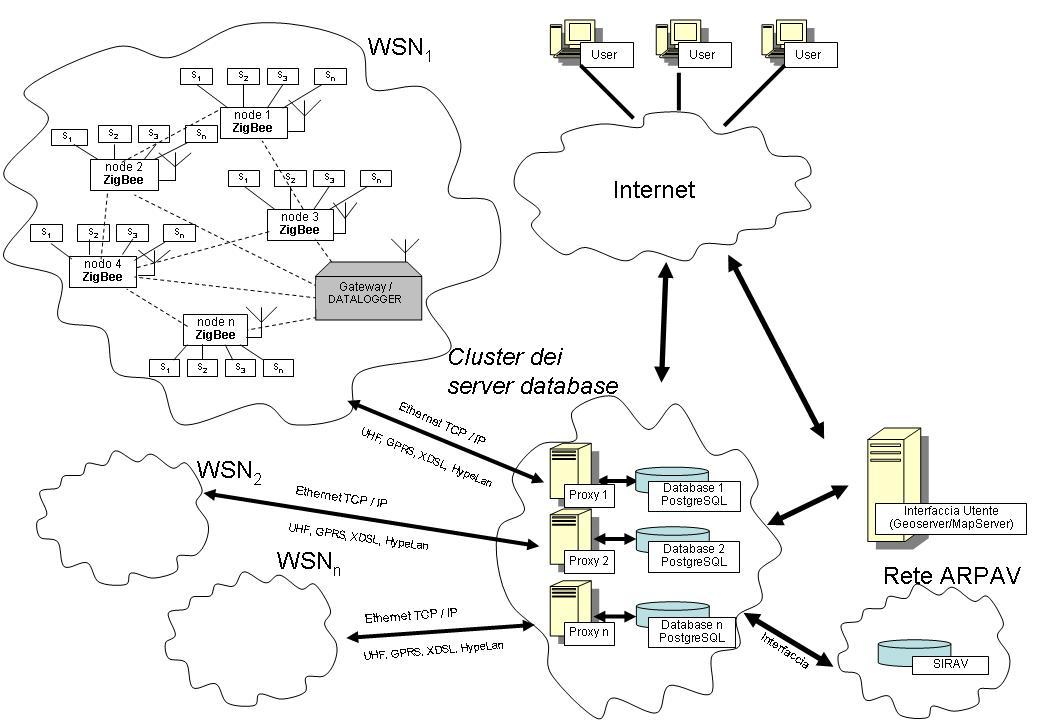
\includegraphics[scale=0.3]{./capitoli/capitolo1/img/retiresmia}
\caption{schema reti RESMIA}
\end{figure}

Il dipartimento di informatica e reti ha il compito di incrementare la struttura del sistema di salvataggio dei dati e di potenziare l'interfaccia \textit{web} che rappresenta graficamente su un'opportuna mappa la dislocazione dei sensori e ed effettuare opportune interrogazioni sui dati forniti tramite \textit{Map Server}\ped{g}.

\subsection{I Servizi di ARPAV}

L'agenzia regionale offre una vasta gamma di servizi, i quali possono essere suddivisi in due macro categorie: servizi ambientali e servizi online. I primi, offrono un servizio su richiesta o erogati da ARPAV, i secondi invece sono servizi passivi offerti dal portale \textit{internet}, i cui fruitori possono accedervi tramite \textit{network}.  \textit{\href{http://www.arpa.veneto.it/servizi-ambientali}{website}}

\subsubsection{Servizi Ambientali}

\begin{longtable}{ p{0.3\textwidth} | p{0.3\textwidth} | p{0.4\textwidth}}
\textbf{Nome}& \textbf{Possibili Fruitori}&  \textbf{Descrizione} \\
\endhead

	\midrule
	\textbf{{\color{OliveGreen}Acquisti pubblici verdi-GPP\ped{g}}} & Pubbliche amministrazioni locali o nazionali  & Informazione delle pubbliche amministrazioni circa l'adozione di pratiche d'acquisto verdi che riducono l'uso di risorse naturali, la produzione di rifiuti, i rischi ambientali \\
	\midrule
	\textbf{{\color{OliveGreen}Certificazioni ambientali}} & Imprese soprattutto piccole e medie &  Diffusione all'interno del mondo produttivo di una nuova cultura di sistema per la gestione consapevole ed ecocompatibile dell'ambiente attraverso lo sviluppo di progetti, strumenti, protocolli ad hoc\\
	\midrule
	\textbf{{\color{OliveGreen}Comunicazione}} & Cittadini & Promozione delle attività di educazione ed informazione ambientale dei cittadini \\
	\midrule
	\textbf{{\color{OliveGreen}Progetti \& Cooperazione}} & Aziende, imprese, enti pubblici o regioni & Avvio e realizzazione di progetti, avvio di relazioni internazionali generalmente finanziati da fondi dell'Unione Europea \\
	\midrule
	\textbf{{\color{OliveGreen} Grandi opere}} & Aziende coinvolte in appalti pubblici in Veneto & attività di audit preventivo e di monitoraggio ambientale per garantire la compatibilità ambientale, il corretto inserimento dal punto di vista urbanistico, ambientale, trasportistico e sociale delle Grandi Opere \\
	\midrule
	\textbf{{\color{OliveGreen} Educazione per la sostenibilità}} & Chiunque &  Attività di educazione, informazione e comunicazione ambientale, protezione della natura al fine di promuovere e sviluppare comportamenti sostenibili \\
	\midrule
	\textbf{{\color{OliveGreen} IPPC\ped{g} e  Servizi alle aziende}} & Aziende ed Imprese & Consulenze sul piano di monitoraggio e controllo in fase istruttoria per il rilascio dell'autorizzazione integrata ambientale, ispezioni integrate ambientali nelle aziende IPPC del Veneto\\
	\midrule
	\textbf{{\color{OliveGreen} Pronta disponibilità}} &  Dipartimenti di Prevenzione delle ULSS regionali Organi di polizia giudiziaria &  Attività di analisi immediata di aria, acqua e suolo secondo le modalità previste\\
	\midrule
	\textbf{{\color{OliveGreen} Rischio industriale}} & Industrie & Individuazione, classificazione e probabilità dei pericoli provenienti dalle industrie che utilizzano o detengono sostanze chimiche per le loro attività \\
	\midrule
	\textbf{{\color{OliveGreen} Sicurezza impiantistica}} & Comuni, ASL, Prefettura, Procura & Verifica della corretta funzionalità di impianti e macchinari installati in ambienti di lavoro o di vita e soggetti a controlli periodici \\
	\bottomrule
	

\caption{servizi ambientali ARPAV}
\end{longtable}

\subsubsection{Servizi Online}

\begin{longtable}{p{0.3\textwidth}|p{0.7\textwidth}}
\textbf{Nome} & \textbf{Descrizione} \\
\endhead

\midrule
\textbf{{\color{Plum} Accesso informazioni ambientali}} & Accesso del pubblico all'informazione ambientale detenuta o prodotta da soggetti pubblici avviene anche mediante l'utilizzo delle tecnologie informatiche e dei mezzi di telecomunicazione \\
\midrule
\textbf{{\color{Plum} Glossari Ambientali}} & Strumento di informazione aggiornata ed esaustiva che ARPAV mette a disposizione dei cittadini per favorire la comprensione di termini 'ambientali' maggiormente utilizzati \\
\midrule
\textbf{{\color{Plum} Iscrizione bollettini}} & Iscrizione alla mailing list consente di ricevere i bollettini Meteo direttamente nella propria casella di posta elettronica. Meteo Veneto, Dolomiti Meteo, Meteo Spiagge e Meteo Garda i bollettini per cui è disponibile il servizio \\
\midrule
\textbf{{\color{Plum} Iscrizione bollettini via sms}} & Sottoscrivendo un abbonamento è possibile ricevere via sms i contenuti di alcuni bollettini prodotti per l'area delle Dolomiti. Dolomiti meteo e Dolomiti Neve e Valanghe i bollettini per i quali è disponibile il servizio \\
\midrule
\textbf{{\color{Plum} Iscrizione \textit{newsletter}}} &  E' possibile ricevere periodicamente nella propria casella di posta le \textit{newsletter} con informazioni su eventi, contenuti e attività \\
\midrule
\textbf{{\color{Plum} Iscrizione applicativo web ORSO }} &  Programma per il monitoraggio del flusso dei rifiuti attraverso le Regioni d'Italia, con standard di riferimento comuni che garantiscano rappresentatività delle informazioni raccolte, oltre ad agevolare lo scambio di informazioni finalizzato alla corretta gestione dei rifiuti per i Comuni e gestori degli impianti \\
\midrule
\textbf{{\color{Plum} Iscrizione a IRRIFRAME}} & Servizio che permette alle aziende registrate di salvare il proprio profilo colturale e di personalizzare l'informazione irrigua fornita dal servizio comunicando in tempo reale dati locali \\
\midrule
\textbf{{\color{Plum} Link utili}} & Una rassegna di 'siti utili'; la suddivisione per argomenti e temi permette di individuare facilmente i riferimenti cercati \\
\midrule
\textbf{{\color{Plum} Richiesta pubblicazioni}} & Possibilità di richiedere una copia delle pubblicazioni edite da ARPAV attraverso posta elettronica e la compilazione di un modulo \\
\bottomrule

\caption{servizi online di ARPAV}
\end{longtable}

\newpage

\section{Organizzazione Interna}

ARPAV è un'agenzia regionale che lavora per il completamento di progetti a livello regionale, nazionale ed internazionale ed offre tutta una serie di servizi a livello regionale e non. Per fare ciò necessita di una  organizzazione interna ben strutturata, suddivisa in vari organi operativi, ognuno dei quali ricopre una funzionalità specifica e si interfaccia con un altra secondo protocolli prestabiliti. ARPAV è dotata di una autonomia interna negli ambiti amministrativi, organizzativi e tecnico contabile e di diverse figure professionali che garantiscono un approccio multidisciplinari.

\begin{figure}[htbp]
\centering
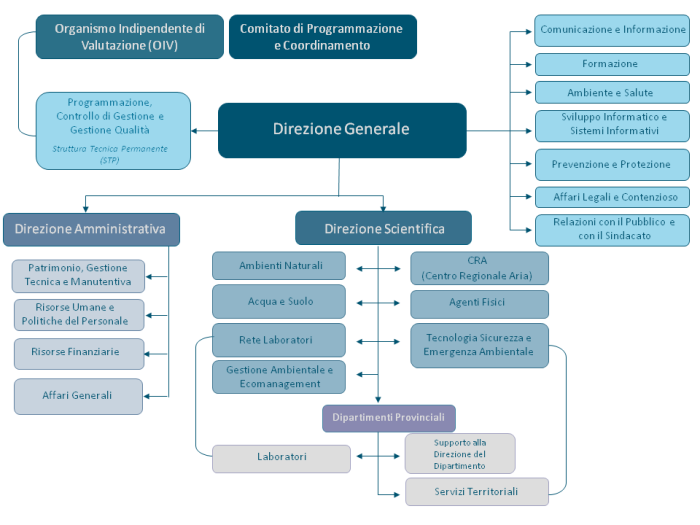
\includegraphics[scale=0.7]{./capitoli/capitolo1/img/organigramma}

\caption{organigramma struttura ARPAV}

\end{figure}

A livello macroscopico è composta da una \textbf{Direzione Generale}, che a sua volta si ramifica in più aree funzionali di natura amministrativa e tecnico-scientifica, due \textbf{Dipartimenti regionali} e sette \textbf{Dipartimenti provinciali}. I dipartimenti regionali e provinciali per la realizzazione dei programmi ed attività di competenza godono di una autonomia gestionale nei limiti delle risorse loro assegnate dalla direzione generale.\\
La sede dello stage si trova all'interno dell'area della \textbf{direzione amministrativa}, in particolare nel sottoinsieme della \textbf{gestione tecnica}.\\
L'organizzazione interna al dipartimento di informatica è riassumibile così:

\begin{figure}[htbp]
	\centering
	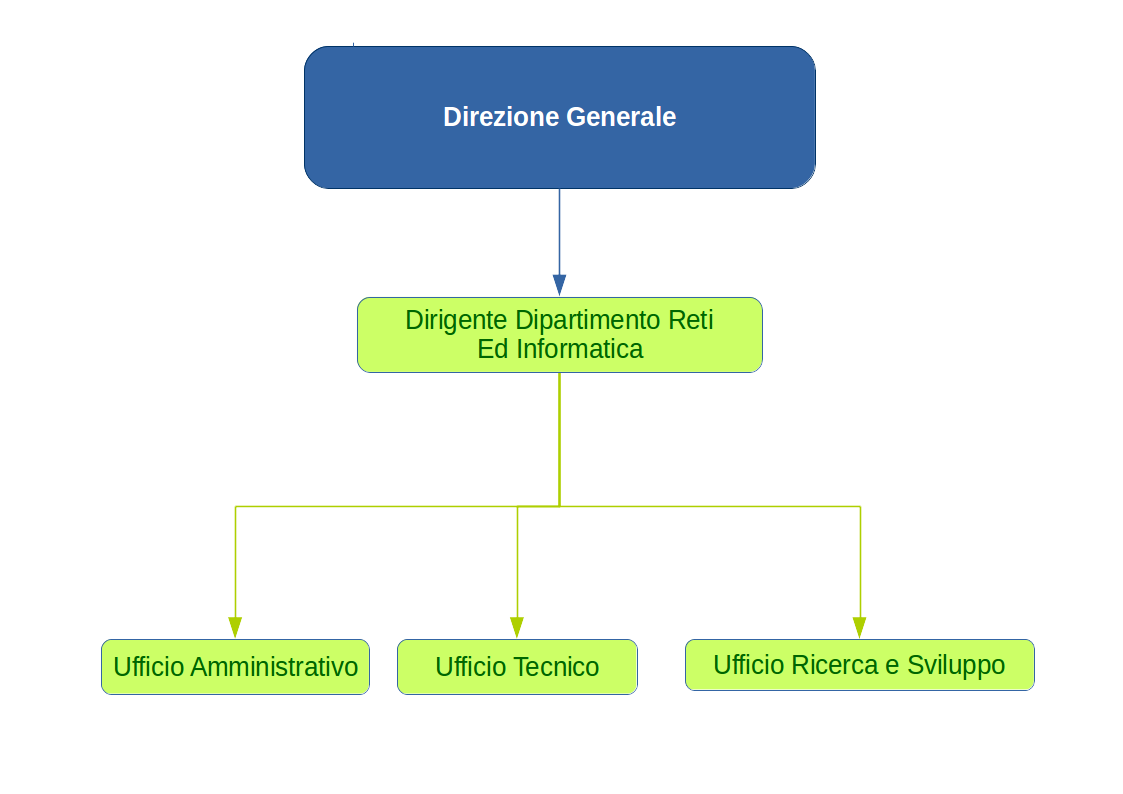
\includegraphics[scale=0.4]{./capitoli/capitolo1/img/organigrammaDip}
	\caption{organigramma Dipartimento Informatica e Reti}
\end{figure}

\begin{itemize}

	\item \textbf{Direttore:} figura a cui tutti fanno riferimento, ha il compito di relazionarsi con le aziende esterne per accordare collaborazioni nei progetti assegnati dalla \textbf{Direzione Generale}. Deve anche approvare i bilanci economici e gestire le risorse umane;
	\item \textbf{Ufficio Amministrativo:} ufficio con il compito di adempiere alle funzioni amministrative del dipartimento;
	\item \textbf{Ufficio di Ricerca e Sviluppo:} ufficio esecutivo in cui si sviluppano o si fa manutenzione sui progetti;
	\item \textbf{Ufficio Tecnico:} ufficio composto da tecnici addetti alla manutenzione del sistema di reti dell'intero ente.
	
\end{itemize}
\subsection{Processi di Sviluppo}


I processi di sviluppo all'interno di  ARPAV non possono essere facilmente standardizzati, in quanto ogni settore operativo ha necessità di agire in modo differente rispetto gli altri. Ogni dipartimento organizza i propri processi in base alla propria funzione e necessità, restando conforme alle linee guida dettate dalla \textbf{Direzione Centrale} tramite i seguenti documenti: 

\begin{itemize}
	\item \textbf{\textit{Piano Triennale Regionale di Educazione Ambientale}}: documento di validità triennale, aggiornato annualmente, in cui si definiscono le linee guida dell'agenzia, gli obiettivi da raggiungere e me metodologie di crescita;
	\item \textbf{\textit{Documento di Programmazione per l'Informazione, la Formazione e l'Educazione Ambientale (IN.F.E.A.)}}: documento in cui vengono definiti provvedimenti, progetti (di durata pluriennale) e le azioni che mirano all'adempimento degli obiettivi prefissati dal Piano Triennale di Educazione Ambientale;
	\item \textbf{\textit{Programma Triennale per la Trasparenza e Integrità}}: documento di validità triennale, aggiornato annualmente, in cui vengono definiti i processi per garantire un livello di trasparenza, legalità e sviluppo della coltura dell'integrità.
	
	
\end{itemize}

\begin{figure}[htpb]
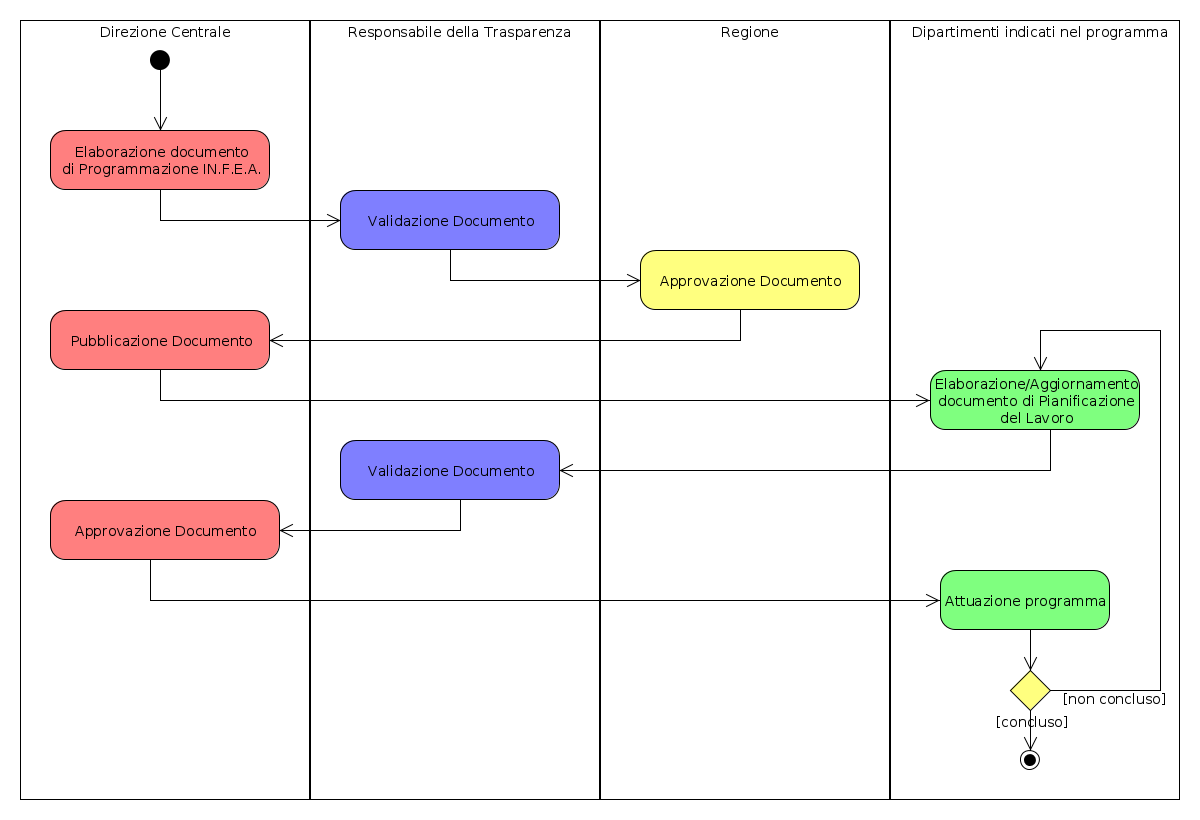
\includegraphics[scale=0.33]{./capitoli/capitolo1/img/attivita_programma}
\caption{diagramma attività approvazione progetti}
\end{figure}

Nel documento di Programmazione IN.F.E.A. vengono determinate le finalità che i progetti triennali intendono perseguire. E' compito dei dipartimenti a cui è stata delegata la realizzazione del progetto, dichiarare la gestione del \textit{budget}, gli interventi di aziende private esterne e la pianificazione degli obiettivi intermedi, tramite la elaborazione, o aggiornamento, di un documento denominato \textit{Pianificazione del Lavoro}. Al suo interno vengono definite le \textit{milestone} che si intendono raggiungere alla fine di ogni anno e, in particolare, la suddivisione del lavoro su base annuale. Il documento viene quindi aggiornato in tre occasioni:

\begin{itemize}
	\item Inizio anno: vengono definiti i traguardi che si realizzeranno durante l'anno in corso, le ore preventivate per attività e il \textit{budget} che si presume di spendere;
	\item Dopo sei mesi: viene aggiornato lo stato di avanzamento del progetto con relative modifiche;
	\item Fine anno: viene aggiornato lo stato di avanzamento del progetto con relative modifiche del piano di lavoro triennale e ci si predispone la stesura del successivo anno di lavoro o la conclusione del progetto stesso.
\end{itemize}

Ogni incremento del documento viene visionato dal responsabile della trasparenza e approvato dalla Direzione Centrale.



In particolare, nel dipartimento sede dello \textit{stage}, dovendo lavorare su progetti informatici ampi e complessi, l'approccio utilizzato è di tipo \textit{top-down}. Progetti che coinvolgono l'impiego di risorse per periodi duraturi, richiedono una accurata e solida conoscenza delle problematiche che si devono affrontare e, in particolare, una robusta ed accurata progettazione. Tramite questo processo si suddivide un problema complesso in sottoproblemi più semplici. Ogni sottoproblema è descritto in modo dettagliato e, se complesso, a sua volta può essere suddiviso ulteriormente.

\begin{figure}[htpb]
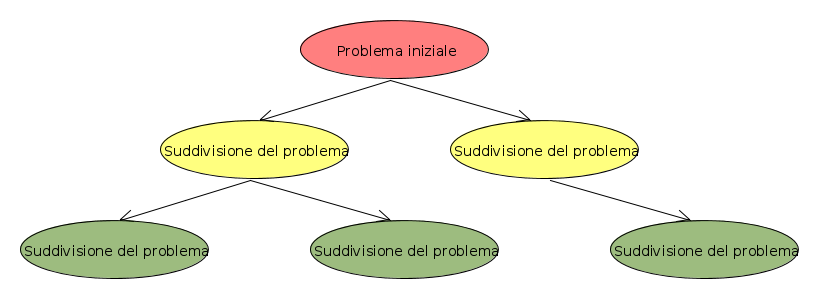
\includegraphics[scale=0.5]{./capitoli/capitolo1/img/probo}
\caption{raffigurazione divisione problema approccio top-down}
\end{figure}

Vantaggi \textit{top-down}:
\begin{itemize}
\item \textbf{Semplificazione del problema:} la suddivisione di un problema complesso in più sottoproblemi permette di trovare soluzioni efficientemente;
\item \textbf{Suddivisione dei compiti:} la suddivisione dei problemi permette una programmazione parallela dei sottoproblemi indipendenti fra loro;
\item \textbf{Programmazione semplificata:} una volta conclusa la programmazione, l'attività di programmazione risulterà semplice poiché si limiterà alla trascrizione in codice della progettazione ampiamente dettagliata;
\item \textbf{Comprensione più semplice:} dividendo il problema in più parti rende più semplice la comprensione del lavoro, così da facilitarne una manutenzione futura.

\end{itemize}
 
Svantaggi \textit{top-down}:

\begin{itemize}

\item \textbf{Fase di test:} non esistendo un eseguibile fino alla quasi conclusione del progetto, eseguire test può risultare complicato;
\item \textbf{Scarse relazioni:} un approccio \textit{top-down} sfavorisce le interazioni con gli \textit{stakeholder}, in quanto devono attendere fino alle ultime fasi del progetto per visualizzare prototipi o bozze del progetto.
\end{itemize}

Il modello di ciclo di vita del \textit{software} utilizzato è un modello a cascata, nel quale si prediligono delle fasi ben distinte di lavoro. Ogni fase ha un \textit{input} di inizio e un \textit{output} di fine, il quale è l'\textit{input} fase successiva.

\begin{figure}[htbp]
	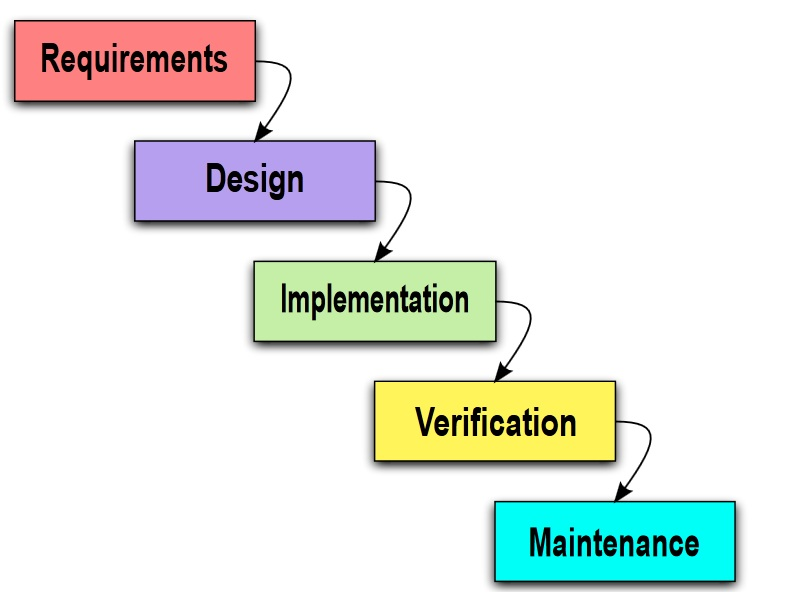
\includegraphics[scale=0.3]{./capitoli/capitolo1/img/cascata}
	\caption{ciclo di vita a cascata}

\end{figure}

Dalla presentazione di un problema o un'opportunità (\textit{input}), si inizia una fase di \textit{analisi}, nella quale si studiano a fondo i problemi presentati e si produce un documento di \textit{Analisi dei Requisiti} (\textit{output)}. Successivamente si procede con la progettazione, finita la quale, si inizia con la codifica e test. Conclusa quest'ultima fase si passa alla verifica  e validazione ed infine, con il rilascio del prodotto, si procede con la manutenzione.

 
\subsection{Metodologie di Supporto ai Processi}

Di seguito vengono riportate le metodologie del dipartimento sede \textit{stage}.

\subsubsection{Analisi dei Requisiti}

In questa fase si prende visione del o dei progetti assegnati dalla Direzione Centrale tramite il documento di di Programmazione IN.F.E.A. . Gli analisti, interni o in caso di necessità esterni, sono gli attori principali per tutto questo periodo. Vengono studiati attentamente i capitolati e riportati tramite diagrammi \textit{use case} le funzionalità riscontrate. In questa fase vengono effettuati studi per la ricerca di \textit{patner} nel progetto. Eventualmente possono essere eseguiti rilievi su campo per approfondire ulteriormente i dati ambientali in possesso. Il responsabile del dipartimento ha il compito di visionare questa fase scrupolosamente, poiché dovrà approvare o meno scelte che graveranno sul totale del bilancio, ponendo molta attenzione a non sforare il \textit{budget} a disposizione. Se necessario la fase di analisi può essere delegata a terzi.

\subsubsection{Progettazione}

Per la progettazione viene prima identificata una architettura generale ad alto livello che viene poi sviluppata in maggior dettaglio. Questa fase è cruciale per la riuscita del progetto. Il responsabile del dipartimento, se ritenuto necessario, può richiedere l'intervento di aiuti esterni per consultazioni specifiche.

\subsubsection{Realizzazione e Test}

Durante questa fase il responsabile del dipartimento ha un ruolo marginale, in quanto il lavoro di codifica non richiede particolare consumo di risorse, e si limita all'assegnazione dei compiti attraverso un sistema di \textit{ticketing} per favorire una codifica in parallelo. Durante questa fase sono richiesti molti stagisti.

\subsubsection{Manutenzione}

Gran parte del lavoro che avviene all'interno del dipartimento di reti e informatica è di manutenzione. Vengono aperti costantemente \textit{ticket} per la manutenzione di vecchi progetti e servizi. Il responsabile del dipartimento ha il compito  ascoltare relative lamentele da parte degli usufruttuari dei servizi o prodotti, organizzare riunioni col team per la risoluzione dei problemi riscontrati e la suddivisione dei lavori di manutenzione. 

\subsection{Strumenti di Supporto ai Processi}

\subsubsection{Gestione Documenti}
La documentazione di analisi dei requisiti e di progettazione è raccolta all'interno di \textit{repository} gestite dai loro \textit{server}, accessibili attraverso loro \textit{network}. Per altri documenti vengono usati servizi di \textit{Google} come \textit{Google Drive}.

\subsubsection{Ticketing}

Durante la mia presenza in sede di \textit{stage}, ho notato che gli strumenti di \textit{ticketing}, per quanto venissero utilizzati per la maggior parte delle comunicazioni, era spesso necessario organizzare riunioni straordinarie avvisando gli interessati tramite comunicazioni via \textit{mail}. 

\subsubsection{Gestione Versionamento}

A supporto della fase di codifica viene utilizzato \textit{GitHub} o \textit{Bitbucket}. A seconda della tipologia del progetto possono essere necessarie \textit{repository} private, quindi a pagamento, o pubbliche.

\subsubsection{Gestione Calendario}

Per la gestione delle attività di gruppo, come riunioni ufficiali per il resoconto delle attività o la risoluzione di conflitti interni, viene utilizzato lo strumento \textit{Google Calendar} e il gruppo di \textit{mailing list} interni ai \textit{server} ARPAV per comunicazioni importanti.







\section{Relazioni Esterne}


Essendo un'agenzia regionale finalizzata al monitoraggio e alla tutela dell'ambiente, ARPAV non ha un vero e proprio \textit{target} di clientela. \\
A seconda del ruolo che l'agenzia ricopre in un progetto (\textit{patner} o \textit{leader}) può collaborare con altre agenzie o aziende per fornire prodotti o migliorare infrastrutture. Altrimenti, attraverso i suoi servizi, può interfacciarsi con le singole imprese, industrie e  privati cittadini. 

\subsection{Orientamento all'Innovazione}
Il ruolo di ARPAV si può sintetizzare nelle seguenti parole chiave:
\begin{itemize}


\item Promozione e sostegno
delle attività di informazione ed educazione ambientale dei cittadini, attraverso:
\begin{itemize}
\item Coordinamento delle iniziative a livello regionale per la realizzazione di una rete di soggetti e di riferimenti, con lo scopo di ricercare sinergie ed economie di scala;
\item Formazione dei progettisti di azioni educative e dei formatori/educatori;
\item Monitoraggio e valutazione degli interventi;
\item Accreditamento di progetti di educazione ambientale.
\end{itemize}

\item Gestione delle iniziative di educazione ambientale, attraverso:
\begin{itemize}

\item Gestione diretta di iniziative di formazione e di educazione ambientale;
\item  Compartecipazione ad iniziative gestite da altri soggetti attraverso diverse modalità;
\item  Diffusione e divulgazione delle informazioni ambientali.

\end{itemize}
\end{itemize}
La \textit{mission} di ARPAV si può quindi riassumere in:
\begin{quotation}

\textit{Promuovere la crescita culturale della comunità regionale in termini di conoscenza, capacità, attitudini, motivazioni ed impegno morale, con lo scopo di contribuire individualmente e collettivamente a sostenere un ambiente salutare}
\begin{flushright}
Tratto  \textit{Piano Triennale Regionale di Educazione Ambientale 2001-2003 }
\end{flushright}
\end{quotation}

Fare educazione ambientale e non semplice didattica necessita di focalizzare obiettivi e metodologie da adottare ben precisi. L'Agenzia, per entrare in azione nel modo più efficiente ed efficace possibile, adotta un piano articolato che risponde alle politiche di breve e medio periodo.

Le principali motivazioni che hanno portato l'Agenzia a questa scelta di fondo sono:
\begin{itemize}
\item Avere una visione globale;
\item Condividere obiettivi comuni;
\item Ricercare l'integrazione e le sinergie tra i numerosi soggetti attori, ognuno con una sua specificità ed un suo ruolo preciso;
\item Distribuire in maniera ragionata ed efficiente gli interventi.
\end{itemize}

ARPAV utilizza un processo di qualità \textit{PDCA} per un costante miglioramento.

\begin{figure}[htbp]
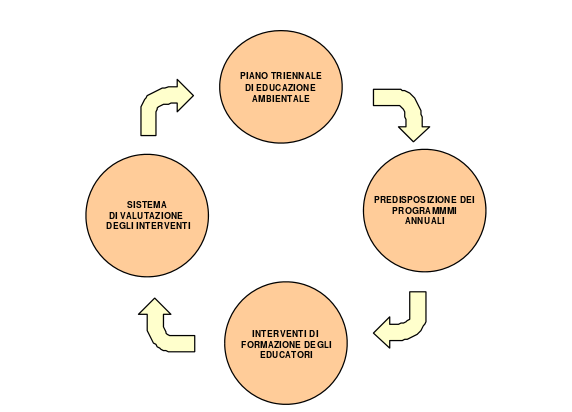
\includegraphics[scale=0.8]{./capitoli/capitolo1/img/pdca}
	\caption{ciclo di \textit{Deming} ARPAV}
\end{figure}
\begin{itemize}

\item \textbf{Predisposizione del piano triennale di educazione ambientale}:
la redazione di un piano triennale, con caratteristiche di piano-processo, soggetto quindi a verifiche periodiche ed ai successivi adeguamenti, implica l'identificazione dei bisogni educativi della popolazione veneta e la conseguente scelta di obiettivi e strategie mirati a perseguire gli stessi. Tale operazione consente di garantire il massimo risultato delle azioni ARPAV perché identifica ed analizza le stesse in termini di costo-beneficio. Inoltre, prevede l'identificazione delle iniziative presenti sul territorio veneto, al fine di favorirne il coordinamento, nonché il coinvolgimento dei vari soggetti, stimolando il loro contributo in forma univoca e mirata ad identificati obiettivi;

\item \textbf{Predisposizione dei programmi di attività annuali:}
il piano triennale conterrà le linee guida per la predisposizione dei programmi di attività annuali, che consentono visibilità e trasparenza delle scelte effettuate e l'integrazione di tutte le energie ARPAV verso traguardi esplicitati. Nel documento vengono descritti progetti e azioni mirate sul campo che prevedono l'attuazione del piano di educazione;

\item \textbf{Interventi di formazione dei progettisti di azioni educative e di formatori/educatori:}
è importante garantire la preparazione di operatori che potranno in tutto il territorio regionale progettare interventi educativi in modo corretto e coerente con l'impostazione ARPAV. Ciò garantirà il massimo beneficio degli interventi stessi perché metodologicamente corretti ed integrati tra di loro. L'acquisizione di abilità metodologiche va considerato come un investimento perché tali operatori potranno incidere per un lungo tempo a venire.

\item \textbf{Creazione di un sistema di monitoraggio e valutazione degli interventi:}
Il piano prevede la creazione di un sistema di monitoraggio e valutazione degli interventi che verranno realizzati: indicatori, sistema informativo, criteri di valutazione, rapporti e loro destinatari.

\end{itemize}